% Generated by Sphinx.
\def\sphinxdocclass{report}
\documentclass[letterpaper,10pt,english]{sphinxmanual}
\usepackage[utf8]{inputenc}
\DeclareUnicodeCharacter{00A0}{\nobreakspace}
\usepackage[T1]{fontenc}
\usepackage{babel}
\usepackage{times}
\usepackage[Bjarne]{fncychap}
\usepackage{longtable}
\usepackage{sphinx}
\usepackage{multirow}


\title{RBAC-SLR Documentation}
\date{February 02, 2013}
\release{0.1}
\author{Eric D. Helms}
\newcommand{\sphinxlogo}{}
\renewcommand{\releasename}{Release}
\makeindex

\makeatletter
\def\PYG@reset{\let\PYG@it=\relax \let\PYG@bf=\relax%
    \let\PYG@ul=\relax \let\PYG@tc=\relax%
    \let\PYG@bc=\relax \let\PYG@ff=\relax}
\def\PYG@tok#1{\csname PYG@tok@#1\endcsname}
\def\PYG@toks#1+{\ifx\relax#1\empty\else%
    \PYG@tok{#1}\expandafter\PYG@toks\fi}
\def\PYG@do#1{\PYG@bc{\PYG@tc{\PYG@ul{%
    \PYG@it{\PYG@bf{\PYG@ff{#1}}}}}}}
\def\PYG#1#2{\PYG@reset\PYG@toks#1+\relax+\PYG@do{#2}}

\expandafter\def\csname PYG@tok@gd\endcsname{\def\PYG@tc##1{\textcolor[rgb]{0.63,0.00,0.00}{##1}}}
\expandafter\def\csname PYG@tok@gu\endcsname{\let\PYG@bf=\textbf\def\PYG@tc##1{\textcolor[rgb]{0.50,0.00,0.50}{##1}}}
\expandafter\def\csname PYG@tok@gt\endcsname{\def\PYG@tc##1{\textcolor[rgb]{0.00,0.25,0.82}{##1}}}
\expandafter\def\csname PYG@tok@gs\endcsname{\let\PYG@bf=\textbf}
\expandafter\def\csname PYG@tok@gr\endcsname{\def\PYG@tc##1{\textcolor[rgb]{1.00,0.00,0.00}{##1}}}
\expandafter\def\csname PYG@tok@cm\endcsname{\let\PYG@it=\textit\def\PYG@tc##1{\textcolor[rgb]{0.25,0.50,0.56}{##1}}}
\expandafter\def\csname PYG@tok@vg\endcsname{\def\PYG@tc##1{\textcolor[rgb]{0.73,0.38,0.84}{##1}}}
\expandafter\def\csname PYG@tok@m\endcsname{\def\PYG@tc##1{\textcolor[rgb]{0.13,0.50,0.31}{##1}}}
\expandafter\def\csname PYG@tok@mh\endcsname{\def\PYG@tc##1{\textcolor[rgb]{0.13,0.50,0.31}{##1}}}
\expandafter\def\csname PYG@tok@cs\endcsname{\def\PYG@tc##1{\textcolor[rgb]{0.25,0.50,0.56}{##1}}\def\PYG@bc##1{\setlength{\fboxsep}{0pt}\colorbox[rgb]{1.00,0.94,0.94}{\strut ##1}}}
\expandafter\def\csname PYG@tok@ge\endcsname{\let\PYG@it=\textit}
\expandafter\def\csname PYG@tok@vc\endcsname{\def\PYG@tc##1{\textcolor[rgb]{0.73,0.38,0.84}{##1}}}
\expandafter\def\csname PYG@tok@il\endcsname{\def\PYG@tc##1{\textcolor[rgb]{0.13,0.50,0.31}{##1}}}
\expandafter\def\csname PYG@tok@go\endcsname{\def\PYG@tc##1{\textcolor[rgb]{0.19,0.19,0.19}{##1}}}
\expandafter\def\csname PYG@tok@cp\endcsname{\def\PYG@tc##1{\textcolor[rgb]{0.00,0.44,0.13}{##1}}}
\expandafter\def\csname PYG@tok@gi\endcsname{\def\PYG@tc##1{\textcolor[rgb]{0.00,0.63,0.00}{##1}}}
\expandafter\def\csname PYG@tok@gh\endcsname{\let\PYG@bf=\textbf\def\PYG@tc##1{\textcolor[rgb]{0.00,0.00,0.50}{##1}}}
\expandafter\def\csname PYG@tok@ni\endcsname{\let\PYG@bf=\textbf\def\PYG@tc##1{\textcolor[rgb]{0.84,0.33,0.22}{##1}}}
\expandafter\def\csname PYG@tok@nl\endcsname{\let\PYG@bf=\textbf\def\PYG@tc##1{\textcolor[rgb]{0.00,0.13,0.44}{##1}}}
\expandafter\def\csname PYG@tok@nn\endcsname{\let\PYG@bf=\textbf\def\PYG@tc##1{\textcolor[rgb]{0.05,0.52,0.71}{##1}}}
\expandafter\def\csname PYG@tok@no\endcsname{\def\PYG@tc##1{\textcolor[rgb]{0.38,0.68,0.84}{##1}}}
\expandafter\def\csname PYG@tok@na\endcsname{\def\PYG@tc##1{\textcolor[rgb]{0.25,0.44,0.63}{##1}}}
\expandafter\def\csname PYG@tok@nb\endcsname{\def\PYG@tc##1{\textcolor[rgb]{0.00,0.44,0.13}{##1}}}
\expandafter\def\csname PYG@tok@nc\endcsname{\let\PYG@bf=\textbf\def\PYG@tc##1{\textcolor[rgb]{0.05,0.52,0.71}{##1}}}
\expandafter\def\csname PYG@tok@nd\endcsname{\let\PYG@bf=\textbf\def\PYG@tc##1{\textcolor[rgb]{0.33,0.33,0.33}{##1}}}
\expandafter\def\csname PYG@tok@ne\endcsname{\def\PYG@tc##1{\textcolor[rgb]{0.00,0.44,0.13}{##1}}}
\expandafter\def\csname PYG@tok@nf\endcsname{\def\PYG@tc##1{\textcolor[rgb]{0.02,0.16,0.49}{##1}}}
\expandafter\def\csname PYG@tok@si\endcsname{\let\PYG@it=\textit\def\PYG@tc##1{\textcolor[rgb]{0.44,0.63,0.82}{##1}}}
\expandafter\def\csname PYG@tok@s2\endcsname{\def\PYG@tc##1{\textcolor[rgb]{0.25,0.44,0.63}{##1}}}
\expandafter\def\csname PYG@tok@vi\endcsname{\def\PYG@tc##1{\textcolor[rgb]{0.73,0.38,0.84}{##1}}}
\expandafter\def\csname PYG@tok@nt\endcsname{\let\PYG@bf=\textbf\def\PYG@tc##1{\textcolor[rgb]{0.02,0.16,0.45}{##1}}}
\expandafter\def\csname PYG@tok@nv\endcsname{\def\PYG@tc##1{\textcolor[rgb]{0.73,0.38,0.84}{##1}}}
\expandafter\def\csname PYG@tok@s1\endcsname{\def\PYG@tc##1{\textcolor[rgb]{0.25,0.44,0.63}{##1}}}
\expandafter\def\csname PYG@tok@gp\endcsname{\let\PYG@bf=\textbf\def\PYG@tc##1{\textcolor[rgb]{0.78,0.36,0.04}{##1}}}
\expandafter\def\csname PYG@tok@sh\endcsname{\def\PYG@tc##1{\textcolor[rgb]{0.25,0.44,0.63}{##1}}}
\expandafter\def\csname PYG@tok@ow\endcsname{\let\PYG@bf=\textbf\def\PYG@tc##1{\textcolor[rgb]{0.00,0.44,0.13}{##1}}}
\expandafter\def\csname PYG@tok@sx\endcsname{\def\PYG@tc##1{\textcolor[rgb]{0.78,0.36,0.04}{##1}}}
\expandafter\def\csname PYG@tok@bp\endcsname{\def\PYG@tc##1{\textcolor[rgb]{0.00,0.44,0.13}{##1}}}
\expandafter\def\csname PYG@tok@c1\endcsname{\let\PYG@it=\textit\def\PYG@tc##1{\textcolor[rgb]{0.25,0.50,0.56}{##1}}}
\expandafter\def\csname PYG@tok@kc\endcsname{\let\PYG@bf=\textbf\def\PYG@tc##1{\textcolor[rgb]{0.00,0.44,0.13}{##1}}}
\expandafter\def\csname PYG@tok@c\endcsname{\let\PYG@it=\textit\def\PYG@tc##1{\textcolor[rgb]{0.25,0.50,0.56}{##1}}}
\expandafter\def\csname PYG@tok@mf\endcsname{\def\PYG@tc##1{\textcolor[rgb]{0.13,0.50,0.31}{##1}}}
\expandafter\def\csname PYG@tok@err\endcsname{\def\PYG@bc##1{\setlength{\fboxsep}{0pt}\fcolorbox[rgb]{1.00,0.00,0.00}{1,1,1}{\strut ##1}}}
\expandafter\def\csname PYG@tok@kd\endcsname{\let\PYG@bf=\textbf\def\PYG@tc##1{\textcolor[rgb]{0.00,0.44,0.13}{##1}}}
\expandafter\def\csname PYG@tok@ss\endcsname{\def\PYG@tc##1{\textcolor[rgb]{0.32,0.47,0.09}{##1}}}
\expandafter\def\csname PYG@tok@sr\endcsname{\def\PYG@tc##1{\textcolor[rgb]{0.14,0.33,0.53}{##1}}}
\expandafter\def\csname PYG@tok@mo\endcsname{\def\PYG@tc##1{\textcolor[rgb]{0.13,0.50,0.31}{##1}}}
\expandafter\def\csname PYG@tok@mi\endcsname{\def\PYG@tc##1{\textcolor[rgb]{0.13,0.50,0.31}{##1}}}
\expandafter\def\csname PYG@tok@kn\endcsname{\let\PYG@bf=\textbf\def\PYG@tc##1{\textcolor[rgb]{0.00,0.44,0.13}{##1}}}
\expandafter\def\csname PYG@tok@o\endcsname{\def\PYG@tc##1{\textcolor[rgb]{0.40,0.40,0.40}{##1}}}
\expandafter\def\csname PYG@tok@kr\endcsname{\let\PYG@bf=\textbf\def\PYG@tc##1{\textcolor[rgb]{0.00,0.44,0.13}{##1}}}
\expandafter\def\csname PYG@tok@s\endcsname{\def\PYG@tc##1{\textcolor[rgb]{0.25,0.44,0.63}{##1}}}
\expandafter\def\csname PYG@tok@kp\endcsname{\def\PYG@tc##1{\textcolor[rgb]{0.00,0.44,0.13}{##1}}}
\expandafter\def\csname PYG@tok@w\endcsname{\def\PYG@tc##1{\textcolor[rgb]{0.73,0.73,0.73}{##1}}}
\expandafter\def\csname PYG@tok@kt\endcsname{\def\PYG@tc##1{\textcolor[rgb]{0.56,0.13,0.00}{##1}}}
\expandafter\def\csname PYG@tok@sc\endcsname{\def\PYG@tc##1{\textcolor[rgb]{0.25,0.44,0.63}{##1}}}
\expandafter\def\csname PYG@tok@sb\endcsname{\def\PYG@tc##1{\textcolor[rgb]{0.25,0.44,0.63}{##1}}}
\expandafter\def\csname PYG@tok@k\endcsname{\let\PYG@bf=\textbf\def\PYG@tc##1{\textcolor[rgb]{0.00,0.44,0.13}{##1}}}
\expandafter\def\csname PYG@tok@se\endcsname{\let\PYG@bf=\textbf\def\PYG@tc##1{\textcolor[rgb]{0.25,0.44,0.63}{##1}}}
\expandafter\def\csname PYG@tok@sd\endcsname{\let\PYG@it=\textit\def\PYG@tc##1{\textcolor[rgb]{0.25,0.44,0.63}{##1}}}

\def\PYGZbs{\char`\\}
\def\PYGZus{\char`\_}
\def\PYGZob{\char`\{}
\def\PYGZcb{\char`\}}
\def\PYGZca{\char`\^}
\def\PYGZam{\char`\&}
\def\PYGZlt{\char`\<}
\def\PYGZgt{\char`\>}
\def\PYGZsh{\char`\#}
\def\PYGZpc{\char`\%}
\def\PYGZdl{\char`\$}
\def\PYGZti{\char`\~}
% for compatibility with earlier versions
\def\PYGZat{@}
\def\PYGZlb{[}
\def\PYGZrb{]}
\makeatother

\begin{document}

\maketitle
\tableofcontents
\phantomsection\label{index::doc}


Contents:


\chapter{1. Introduction}
\label{intro:introduction}\label{intro:systematic-literature-review-of-rbac-analysis-notes}\label{intro::doc}
Why is the base model of RBAC extended by newer models?

Role-based access control (RBAC) models {\hyperref[intro:ferraiolo-rbac]{{[}1{]}}} become popularly used to govern access to critical resources.  In an RBAC model, roles represent a group of users who are involved in a specific job function in an organization. RBAC assigns permissions of specific actions on resources to roles instead of individual users.  Therefore, in order to gain roles' permission on specific resources, users acquire appropriate roles first.

RBAC is a generalized access control approach used for various applications including web services, database applications, and healthcare applications.  RBAC has advantages in maintaining and managing organization's security policies.  For example, if a user is to access manager role's resources within a given organization, security policy administrators simply add the user to be associated with the manager role.

RBAC is first introduced in 1990s, NIST proposed standard RBAC model {\hyperref[intro:ferraiolo-rbac]{{[}1{]}}}
Standard RBAC model considers only role-user association and role hierarchy.
Since standard RBAC model has limitations such as specifying environmental constraints or context information
Researchers developed extended models of RBAC to overcome the limitations.
However, as researchers often develop their own specialized extended models of RBAC,
their research cannot be generalized or compared with other research work appropriately.
As a result, researchers could take time on reinventing the wheel.
But how do we, as a community, ensure that a metric is suitable and acceptable for its intended purpose?

The goal of this work is to synthesize available research results on extended models of RBAC. We analyze their extended features and claimed research contributions to find limitations of current RBAC models and what extent of extended features by
comparing with similar research work.
We conducted a systematic literature review (SLR) to evaluate and interpret all available research relevant to a particular research question or topic area of interest.
\begin{description}
\item[{Our research give benefits to a community as follows:}] \leavevmode\begin{itemize}
\item {} 
Our work summarizes current extended RBAC research work and its contributions. By synthesizing the current results, our work shows a roadmap of current extended RBAC research.

\item {} 
Our work guides a direction for a standard of extended RBAC. Understanding the categorization and the motivation of the existing research results helps decide a standard of extended RBAC.

\item {} 
Our work shows a criteria in comparison among research results.

\item {} 
Our work helps identify the research challenges in the ares of security policies and suggest a future extension of RBAC.

\end{itemize}

\end{description}




\chapter{2. Methodology and Process}
\label{process:methodology-and-process}\label{process::doc}
For the first phase of our systematic literature review, an automated comprehensive search of multiple academic search engines was performed. The list of search engines were:
\begin{itemize}
\item {} 
Google Scholar - \href{http://scholar.google.com}{http://scholar.google.com}

\item {} 
IEEExplore     - \href{http://ieeexplore.ieee.org}{http://ieeexplore.ieee.org}

\item {} 
ACM Portal     - \href{http://dl.acm.org}{http://dl.acm.org}

\item {} 
CiteSeerX      - \href{http://http://citeseerx.ist.psu.edu/index}{http://http://citeseerx.ist.psu.edu/index}

\end{itemize}

For each of the criteria below, a search was performed on each of the search engines for a total of 12 data sets.  The criteria used were:
\begin{itemize}
\item {} 
role based access control

\item {} 
RBAC

\item {} 
role-based access control

\end{itemize}

The search performed was done in an automated way using a set of scripts to query and collect data from each search engine with the criteria string as input.  For each criteria for each search engine, the results were captured until a stopping criteria was met.  Each run was performed as follows:
\begin{enumerate}
\item {} 
Remote call to search engine with current search start position and the current search criteria.

\item {} 
Parse results and extract paper title, authors and year of publication.

\item {} 
Compare results against stopping criteria.

\end{enumerate}
\begin{itemize}
\item {} 
If stopping criteria met, stop search.

\item {} 
If stopping criteria not met, increase search position by number of results and return to step 1.

\end{itemize}

The stopping criteria used was either after the first 1000 results, a limitation imposed by some of the search engines, or if ten consecutive results did not contain the search criteria phrase within the title.  After gathering all 12 data sets, the data was combined into a master list by systematically comparing the bibliographic information for each.  After producing a master list, a series of assessment rounds were performed to narrow the paper list and identify primary sources.

There were a total of three elimination rounds.  The first round was based solely on title, the second on reading of the abstract and the last round was based on a full read of the paper and comparison to the research questions outlined.  Each round was performed as follows:
\begin{itemize}
\item {} 
Each reviewer independently classified papers as relevant, irrelevant or uncertain.

\item {} 
Those papers marked as relevant by both reviewers were kept and those marked irrelevant by both were thrown out.

\item {} 
Papers marked as relevant, or irrelevant by a single reviewer were combined with all papers marked as uncertain and discussed by both reviewers.  From this discussion, papers were either thrown out or kept until the next round of the review.  Ties were broken by an indepedent party.

\end{itemize}

The results of the searches is summarised below:

\begin{tabulary}{\linewidth}{|L|L|L|L|L|}
\hline
\textbf{
Search Engines
} & \textbf{
RBAC
} & \textbf{
role based access control
} & \textbf{
role-based access control
} & \textbf{
Total
}\\\hline

Google Scholar
 & 
651
 & 
213
 & 
435
 & 
1299
\\\hline

ACM Portal
 & 
500
 & 
20
 & 
720
 & 
1240
\\\hline

IEEExplore
 & 
200
 & 
40
 & 
230
 & 
470
\\\hline

CiteSeerX
 & 
100
 & 
100
 & 
150
 & 
350
\\\hline
 &  &  &  & \\\hline

Totals
 & 
1451
 & 
373
 & 
1535
 & 
3359
\\\hline

Combined
 &  &  &  & 
\textbf{1716}
\\\hline
\end{tabulary}



\section{Research Questions}
\label{process:research-questions}
Based on our intial intent for the systematic literature review, and notes taken during the third phase of elimination, we have identified the following research questions:
\begin{itemize}
\item {} 
RQ1. What are the deficiencies in current RBAC model to propose extended RBAC models?

\item {} 
RQ2. What are the motivations behind RBAC extensions?

\item {} 
RQ3. What are the categorizations of RBAC model proposed?

\item {} 
RQ4. For each categorization, what are the extended features of RBAC model proposed?

\item {} 
RQ5. Do these models have corresponding implementations in practice?

\item {} 
RQ6. How are extended RBAC models evaluated in theory and in practice?

\item {} 
RQ7. Are there any commonalties or generalizations across all categorizations?

\item {} 
RQ8. What domains or scenarios serve as inspiration for these extensions?

\end{itemize}


\chapter{RQ1: What are the deficiencies in current RBAC model?}
\label{research_questions/RQ_1:rq1-what-are-the-deficiencies-in-current-rbac-model}\label{research_questions/RQ_1::doc}

\section{Common Themes}
\label{research_questions/RQ_1:common-themes}\begin{itemize}
\item {} 
\end{itemize}


\section{By Category}
\label{research_questions/RQ_1:by-category}\begin{description}
\item[{Constraint}] \leavevmode\begin{itemize}
\item {} 
no support for partial inheritance

\item {} 
inability to support permission assignment constraints

\end{itemize}

\item[{Context}] \leavevmode\begin{itemize}
\item {} 
Missing ability to apply constraints between role and permissions and enforce

\item {} 
Missing context that defines if a role can be activated at execution time

\item {} 
Role activation on a per object or process execution rather than session based

\item {} 
No allowance for context to check permission at execution moment based on context

\item {} 
activation of roles based on current context rather than session intiation

\item {} 
conflict resolution

\item {} 
RBAC cannot handle dynamic authorization and entities

\item {} 
Role cannot be resource dependent

\item {} 
RBAC is too simple

\item {} 
Missing granularity

\item {} 
Inability to handle dynamic nature of multiple projects with multiple resources

\item {} 
Too simple

\item {} 
Lacks context

\item {} 
Handling authorization between applications and within can be different

\end{itemize}

\item[{Organizational}] \leavevmode\begin{itemize}
\item {} 
RBAC cannot handle cross-organizational roles and access in an administratively easy way

\end{itemize}

\item[{Privacy}] \leavevmode\begin{itemize}
\item {} 
Privacy regulations are complex, with many entities, RBAC lacks ability to handle all of these

\item {} 
Context, conflict detection and resolution

\item {} 
RBAC lacks ability to define purpose

\end{itemize}

\item[{Resource}] \leavevmode\begin{itemize}
\item {} 
No support for multiple security domains

\item {} 
No support for same security, different applications

\item {} 
Lack of flexibility

\end{itemize}

\item[{Spatial}] \leavevmode\begin{itemize}
\item {} 
Lack of contextual information

\item {} 
Role needs a defined schema

\item {} 
Role activation based on context

\item {} 
Giving a permission an operation

\end{itemize}

\item[{Spatio/Temporal}] \leavevmode\begin{itemize}
\item {} 
\end{itemize}

\item[{Task}] \leavevmode\begin{itemize}
\item {} 
Needs an entity to represent a task and connect a role and a permission through it

\item {} 
Need for team and tasks

\item {} 
Need for entity between permission and roles to hold constraint and allow for dynamic situations and entities

\end{itemize}

\item[{Temporal}] \leavevmode\begin{itemize}
\item {} 
RBAC can't handle time based constraints for role enablement

\end{itemize}

\end{description}


\chapter{RQ2: What are the motivations behind RBAC extensions?}
\label{research_questions/RQ_2:rq2-what-are-the-motivations-behind-rbac-extensions}\label{research_questions/RQ_2::doc}

\section{Common Themes}
\label{research_questions/RQ_2:common-themes}\begin{itemize}
\item {} 
Roles, users and permissions need context associations

\item {} 
Location and time constraints as well as contexts needed

\item {} 
RBAC lacks ability to link in objects

\item {} 
RBAC does not handle single user base and multiple organizations/applications

\item {} 
Role enablement based on context

\item {} 
User granting/revoking of roles based on context

\end{itemize}


\section{By Category}
\label{research_questions/RQ_2:by-category}\begin{description}
\item[{Constraint}] \leavevmode\begin{itemize}
\item {} 
No support for partial inheritance

\item {} 
Permission assignment constraints

\end{itemize}

\item[{Context}] \leavevmode\begin{itemize}
\item {} 
Relationship between object and viewer can't be represented

\item {} 
Object content matters

\item {} 
Location and time constraints on the user

\item {} 
Departmental context around access

\item {} 
RBAC does not handle many small services to wrap around them

\item {} 
RBAC lacks security principle enforcement

\item {} 
Lack of specifying context, and permission checks of dynamic evaluation time rules

\item {} 
RBAC is static and lacks ability to handle dynamic authorization and definitions

\item {} 
RBAC ignores context

\item {} 
Role granulatiry not well controlled

\item {} 
Roles should depend on the resources

\item {} 
RBAC cannot handle multiple projects with multiple tasks and differing roles in each system but the same user

\item {} 
Lack of context support

\item {} 
Too simple for dynamic environments

\end{itemize}

\item[{Delegation}] \leavevmode\begin{itemize}
\item {} 
Support cross-domain delegation

\end{itemize}

\item[{Organizational}] \leavevmode\begin{itemize}
\item {} 
Reduce administrative complexity of RBAC for multi-organizational

\end{itemize}

\item[{Privacy}] \leavevmode\begin{itemize}
\item {} 
Lack of components, purpose binding, conditions, obligations to handle privacy needs

\end{itemize}

\item[{Resource}] \leavevmode\begin{itemize}
\item {} 
Need to support multiple securtiy domains

\item {} 
Need to support same security with different applications

\item {} 
Role heirarchy adds complexity and reduces flexibility

\end{itemize}

\item[{Spatial}] \leavevmode\begin{itemize}
\item {} 
Lack of contextual information with roles, users and permissions

\item {} 
Role needs a schema to allow specification of attributes

\item {} 
Location based security scenarios

\item {} 
Role activation based on location

\item {} 
Support physical and logical locations

\item {} 
Attaching operations to permissions

\end{itemize}

\item[{Spatio/Temporal}] \leavevmode\begin{itemize}
\item {} 
RBAC doesn't inherently support location and time constraints

\item {} 
Spatial and temporal awareness of roles, inheritance and permissions

\item {} 
Context mechanisms needed

\item {} 
Physical and logical locations, hybrids

\item {} 
Role assignment based off time and space, as well as permissions

\item {} 
\end{itemize}

\item[{Task}] \leavevmode\begin{itemize}
\item {} 
RBAC can't handle large enterprises with multiple applications and single user base

\item {} 
Security requirements for enterprises (look up these)

\end{itemize}

\item[{Temporal}] \leavevmode\begin{itemize}
\item {} 
Workflow based organizations need time base constraint for role enablement

\end{itemize}

\end{description}


\chapter{RQ3: What are the categorizations of proposed RBAC extensions?}
\label{research_questions/RQ_3:rq3-what-are-the-categorizations-of-proposed-rbac-extensions}\label{research_questions/RQ_3::doc}
Across the papers found, a number of higher level categories emerged that each proposed model fell in to.  Some of these categories had singular primary papers, while others had multiple extension models proposed that were deemed independent of one another.

For each category, the breakdown of the papers for each category is:

\begin{tabulary}{\linewidth}{|L|L|}
\hline
\textbf{
Paper
} & \textbf{
Category
}\\\hline

Alam, M. and Hafner, M. and Breu, R. 2006
 & 
Constraint
\\\hline

Tzelepi, Sofia K. and Koukopoulos, Dimitrios K. and Pangalos, George 2001
 & 
Context
\\\hline

Haibo, SHEN and Fan, HONG 2005
 & 
Context
\\\hline

Damian G. Cholewka and Reinhardt A. Botha and Jan H. P. Eloff 2000
 & 
Context
\\\hline

Huang, X. and Wang, H. and Chen, Z. and Lin, J. 2006
 & 
Context
\\\hline

Motta, G.H.M.B. and Furuie, S.S. 2003
 & 
Context
\\\hline

Bao, Y. and Song, J. and Wang, D. and Shen, D. and Yu, G. 2008
 & 
Context
\\\hline

Yamazaki, W. and Hiraishi, H. and Mizoguchi, F. 2004
 & 
Context
\\\hline

Jian-min, H. and Xi-yu, L. and Hui-qun, Y. and Jun, T. 2008
 & 
Context
\\\hline

Thein, N. and others 2011
 & 
Context
\\\hline

Zou, D. and He, L. and Jin, H. and Chen, X. 2009
 & 
Context
\\\hline

Hasebe, K. and Mabuchi, M. and Matsushita, A. 2010
 & 
Delegation
\\\hline

Zhang, Z. and Zhang, X. and Sandhu, R. 2006
 & 
Organizational
\\\hline

Ni, Q. and Trombetta, A. and Bertino, E. and Lobo, J. 2007
 & 
Privacy
\\\hline

Masoumzadeh, A. and Joshi, J. 2008
 & 
Privacy
\\\hline

Zhao, Y. and Zhao, Y. and Lu, H. 2008
 & 
Resource
\\\hline

Bertino, E. and Catania, B. and Damiani, M.L. and Perlasca, P. 2005
 & 
Spatial
\\\hline

Ray, I. and Kumar, M. and Yu, L. 2006
 & 
Spatial
\\\hline

Hansen, F. and Oleshchuk, V. 2003
 & 
Spatial
\\\hline

Aich, S. and Sural, S. and Majumdar, A. 2007
 & 
Spatio-Temporal
\\\hline

Chen, L. and Crampton, J. 2008
 & 
Spatio-Temporal
\\\hline

Samuel, A. and Ghafoor, A. and Bertino, E. 2007
 & 
Spatio-Temporal
\\\hline

Chandran, S. and Joshi, J. 2005
 & 
Spatio-Temporal
\\\hline

Ray, I. and Toahchoodee, M. 2007
 & 
Spatio-Temporal
\\\hline

Aich, S. and Mondal, S. and Sural, S. and Majumdar, A. 2009
 & 
Spatio-Temporal
\\\hline

Yao, L. and Kong, X. and Xu, Z. 2008
 & 
Task
\\\hline

ZHANG, S. and CHEN, X. and HOU, G. 2009
 & 
Task
\\\hline

Oh, S. and Park, S. 2003
 & 
Task
\\\hline

Joshi, J.B.D. and Bertino, E. and Latif, U. and Ghafoor, A. 2005
 & 
Temporal
\\\hline
\end{tabulary}



\section{By Category}
\label{research_questions/RQ_3:by-category}\begin{description}
\item[{Constraint (1)}] \leavevmode
a limitation or restriction

\item[{Context (8)}] \leavevmode
circumstances in which an event occurs

\item[{Delegation (1)}] \leavevmode
the act of empowering to act for another

\item[{Organizational (1)}] \leavevmode
of or relating to an organization

\item[{Privacy (1)}] \leavevmode
freedom from unauthorized intrusion

\item[{Resource (1)}] \leavevmode
an available supply than be drawn on when needed

\item[{Spatial (3)}] \leavevmode
of or relating to facility in percieving relations in space

\item[{Spatio/Temporal (6)}] \leavevmode
combining space and time

\item[{Task (3)}] \leavevmode
a usually assigned piece of work often to be finished within a certain time

\item[{Temporal (1)}] \leavevmode
of or relating to the sequence of time or to a particular time

\end{description}

{\hfill\scalebox{1.000000}{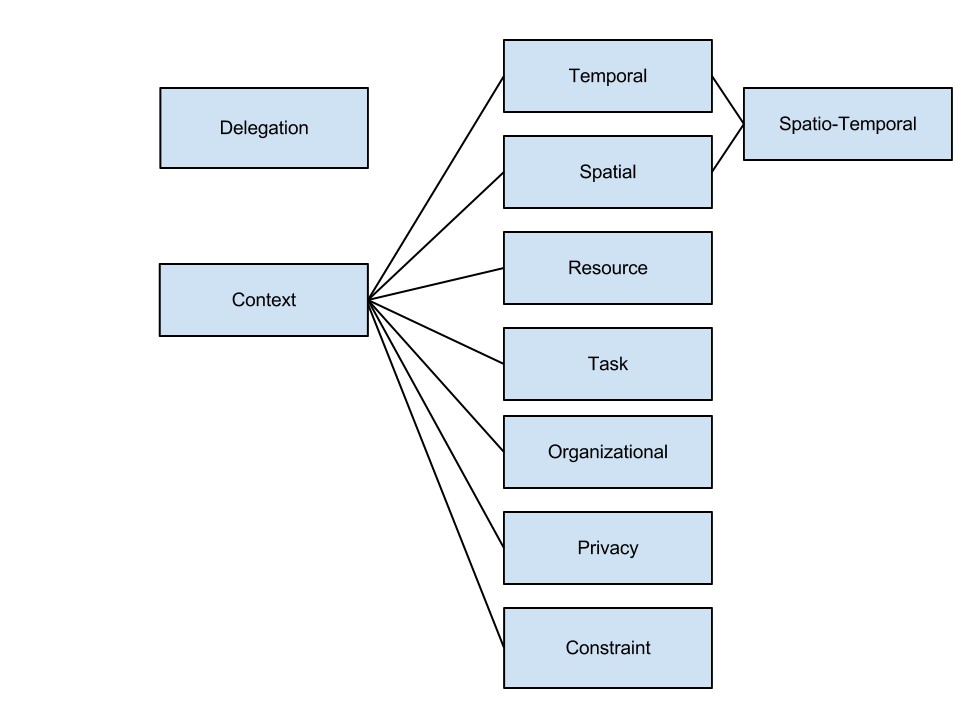
\includegraphics{categories_map.png}}\hfill}


\chapter{RQ4: For each categorization, what are the extended features of RBAC proposed?}
\label{research_questions/RQ_4::doc}\label{research_questions/RQ_4:rq4-for-each-categorization-what-are-the-extended-features-of-rbac-proposed}
Is this the same as RQ\_1 ?


\section{Common Themes}
\label{research_questions/RQ_4:common-themes}\begin{itemize}
\item {} 
\end{itemize}


\section{By Category}
\label{research_questions/RQ_4:by-category}\begin{description}
\item[{Constraint}] \leavevmode\begin{itemize}
\item {} 
\end{itemize}

\item[{Context}] \leavevmode\begin{itemize}
\item {} 
\end{itemize}

\item[{Delegation}] \leavevmode\begin{itemize}
\item {} 
\end{itemize}

\item[{Organizational}] \leavevmode\begin{itemize}
\item {} 
\end{itemize}

\item[{Privacy}] \leavevmode\begin{itemize}
\item {} 
\end{itemize}

\item[{Resource}] \leavevmode\begin{itemize}
\item {} 
\end{itemize}

\item[{Spatial}] \leavevmode\begin{itemize}
\item {} 
\end{itemize}

\item[{Spatio/Temporal}] \leavevmode\begin{itemize}
\item {} 
\end{itemize}

\item[{Task}] \leavevmode\begin{itemize}
\item {} 
\end{itemize}

\item[{Temporal}] \leavevmode\begin{itemize}
\item {} 
\end{itemize}

\end{description}


\chapter{RQ5. Do these models have corresponding implementations in practice?}
\label{research_questions/RQ_5::doc}\label{research_questions/RQ_5:rq5-do-these-models-have-corresponding-implementations-in-practice}
When designing and proposing a model targeted at a feature that is rooted in practical
usage by real software systems, bringing the model to life is strong evidence that the
proposed model can work in practice.  The concept of authorization, and access control
is rooted in a business need.  Thus, any access control model needs to be feasible
in the real world not just on paper.  We analyzed the primary sources to see how many
proposed models actually had implmenetations associated with them.  And quantified the
type of implementation.  Whether the implementation was for a real system, for a prototype
and/or used in a production environment.


\section{Common Themes}
\label{research_questions/RQ_5:common-themes}\begin{itemize}
\item {} 
21 No's

\item {} 
8 Yes's

\item {} 
Half the implementation's were prototypes

\end{itemize}


\section{By Category}
\label{research_questions/RQ_5:by-category}\begin{description}
\item[{Constraint}] \leavevmode\begin{itemize}
\item {} 
No

\end{itemize}

\item[{Context}] \leavevmode\begin{itemize}
\item {} 
No - system architecture provided

\item {} 
No

\item {} 
Yes - prototype with VB6 and MS Access97

\item {} 
Yes - prototype system, system architecture, algorithms implemented, simulation scenarios

\item {} 
Yes - on an EHR system

\item {} 
Yes - prototype using XML container

\item {} 
Yes - web based API agent

\item {} 
No

\item {} 
No

\item {} 
No

\end{itemize}

\item[{Delegation}] \leavevmode\begin{itemize}
\item {} 
No

\end{itemize}

\item[{Organizational}] \leavevmode\begin{itemize}
\item {} 
No

\end{itemize}

\item[{Privacy}] \leavevmode\begin{itemize}
\item {} 
No

\item {} 
No

\end{itemize}

\item[{Resource}] \leavevmode\begin{itemize}
\item {} 
No

\end{itemize}

\item[{Spatial}] \leavevmode\begin{itemize}
\item {} 
No

\item {} 
No

\item {} 
No

\end{itemize}

\item[{Spatio/Temporal}] \leavevmode\begin{itemize}
\item {} 
No

\item {} 
No

\item {} 
No

\item {} 
No

\item {} 
No

\item {} 
Yes - integrated with telemedicine application, web based

\end{itemize}

\item[{Task}] \leavevmode\begin{itemize}
\item {} 
Yes - mentions of systems that exist using the model

\item {} 
Yes - prototype system

\item {} 
No

\end{itemize}

\item[{Temporal}] \leavevmode\begin{itemize}
\item {} 
No

\end{itemize}

\end{description}


\chapter{RQ6. How are extended RBAC models evaluated in theory and in practice?}
\label{research_questions/RQ_6:rq6-how-are-extended-rbac-models-evaluated-in-theory-and-in-practice}\label{research_questions/RQ_6::doc}

\section{Common Themes}
\label{research_questions/RQ_6:common-themes}\begin{itemize}
\item {} 
12 had no evaluation whatsoever

\item {} 
8 present example scenarios and how their model would apply

\item {} 
6 presented performance and time complexity analysis

\end{itemize}


\section{By Category}
\label{research_questions/RQ_6:by-category}\begin{description}
\item[{Constraint}] \leavevmode\begin{itemize}
\item {} 
No evaluation

\end{itemize}

\item[{Context}] \leavevmode\begin{itemize}
\item {} 
Present hospital scenarios and explanation of how new model would handle

\item {} 
No

\item {} 
No

\item {} 
No

\item {} 
No

\item {} 
Scenarios with how model affects, performance test of the model vs. traditional RBAC

\item {} 
Description of a fake project management system that the model is designed for

\item {} 
Applied to conceptual situation

\item {} 
No

\item {} 
Example scenario comparing their model vs other models

\end{itemize}

\item[{Delegation}] \leavevmode\begin{itemize}
\item {} 
No

\end{itemize}

\item[{Organizational}] \leavevmode\begin{itemize}
\item {} 
Comparison caluclation for number of roles vs standard model, numerical size comparisons against other proposed models

\end{itemize}

\item[{Privacy}] \leavevmode\begin{itemize}
\item {} 
Evaluate the performance of permission assignment and authorization checks for various sizes and context variables

\item {} 
No

\end{itemize}

\item[{Resource}] \leavevmode\begin{itemize}
\item {} 
Model comparison from a qualitative standpoint

\end{itemize}

\item[{Spatial}] \leavevmode\begin{itemize}
\item {} 
Algorithm and Big-O performance evaluation

\item {} 
No except minor scenarios and how the model handles

\item {} 
No other than mathematical specification

\end{itemize}

\item[{Spatio/Temporal}] \leavevmode\begin{itemize}
\item {} 
Mathematical description

\item {} 
Mathematical analysis of role graph, complexity comparisons across different models

\item {} 
Pseudo example scenario

\item {} 
No

\item {} 
Detailed scenario with examination of how model handles situation

\item {} 
Discuess difference btween their model and other models, time-complexity analysis to show no performance impact with standard model

\end{itemize}

\item[{Task}] \leavevmode\begin{itemize}
\item {} 
No

\item {} 
No

\item {} 
No

\end{itemize}

\item[{Temporal}] \leavevmode\begin{itemize}
\item {} 
Mathematical modeling and graphs to detail usage and interactions, explanation of example scenarios

\end{itemize}

\end{description}


\chapter{RQ7. Are there any commonalties or generalizations across all categorizations?}
\label{research_questions/RQ_7:rq7-are-there-any-commonalties-or-generalizations-across-all-categorizations}\label{research_questions/RQ_7::doc}

\section{Common Themes}
\label{research_questions/RQ_7:common-themes}\begin{itemize}
\item {} 
\end{itemize}


\section{By Category}
\label{research_questions/RQ_7:by-category}\begin{description}
\item[{Constraint}] \leavevmode\begin{itemize}
\item {} 
\end{itemize}

\item[{Context}] \leavevmode\begin{itemize}
\item {} 
\end{itemize}

\item[{Delegation}] \leavevmode\begin{itemize}
\item {} 
\end{itemize}

\item[{Organizational}] \leavevmode\begin{itemize}
\item {} 
\end{itemize}

\item[{Privacy}] \leavevmode\begin{itemize}
\item {} 
\end{itemize}

\item[{Resource}] \leavevmode\begin{itemize}
\item {} 
\end{itemize}

\item[{Spatial}] \leavevmode\begin{itemize}
\item {} 
\end{itemize}

\item[{Spatio/Temporal}] \leavevmode\begin{itemize}
\item {} 
\end{itemize}

\item[{Task}] \leavevmode\begin{itemize}
\item {} 
\end{itemize}

\item[{Temporal}] \leavevmode\begin{itemize}
\item {} 
\end{itemize}

\end{description}


\chapter{RQ8. What domains or scenarios serve as inspiration for these extensions?}
\label{research_questions/RQ_8:rq8-what-domains-or-scenarios-serve-as-inspiration-for-these-extensions}\label{research_questions/RQ_8::doc}

\section{Common Themes}
\label{research_questions/RQ_8:common-themes}\begin{itemize}
\item {} 
Medical domain

\item {} 
Pervasive computing environments

\item {} 
Mobile devices

\item {} 
Large-scale organizations with many sub-departments

\item {} 
Enterprise, organization workflows

\end{itemize}


\section{By Category}
\label{research_questions/RQ_8:by-category}\begin{description}
\item[{Constraint}] \leavevmode\begin{itemize}
\item {} 
Medical domain

\item {} 
Service Oriented Architecture

\end{itemize}

\item[{Context}] \leavevmode\begin{itemize}
\item {} 
Medical imaging database

\item {} 
Handling an insurance claim workflow

\item {} 
Pervasive computing environments

\item {} 
Medical emergency overrides

\item {} 
Electronic health records

\item {} 
Supermarket

\item {} 
Project management system with large project, task and user base

\item {} 
Power load forecasting system (multi-level user environment)

\end{itemize}

\item[{Delegation}] \leavevmode\begin{itemize}
\item {} 
Large-scale electronic health record systems

\end{itemize}

\item[{Organizational}] \leavevmode\begin{itemize}
\item {} 
Online tutoring system

\item {} 
State education system with schools, districts, etc.

\end{itemize}

\item[{Privacy}] \leavevmode\begin{itemize}
\item {} 
Privacy within the medical domain, HIPAA

\end{itemize}

\item[{Resource}] \leavevmode\begin{itemize}
\item {} 
N/A

\end{itemize}

\item[{Spatial}] \leavevmode\begin{itemize}
\item {} 
Hospital with multi-floors, departments

\end{itemize}

\item[{Spatio/Temporal}] \leavevmode\begin{itemize}
\item {} 
Pervasive computing environments

\item {} 
Hospital using mobile devices with multiple user types on a single floor, departments

\item {} 
Mobile, peer-to-peer

\item {} 
Doctor out in the world needing access during a random medical emergency

\item {} 
Students at a university

\end{itemize}

\item[{Task}] \leavevmode\begin{itemize}
\item {} 
Large enterprises with multiple applications and a single user base

\item {} 
Hospital needs

\item {} 
Complex enterprise environments

\end{itemize}

\item[{Temporal}] \leavevmode\begin{itemize}
\item {} 
General organizational needs for time constraints

\end{itemize}

\end{description}


\chapter{Constraint}
\label{categories/constraint::doc}\label{categories/constraint:constraint}\begin{description}
\item[{Definition}] \leavevmode
a limitation or restriction

\item[{Papers}] \leavevmode\begin{itemize}
\item {} 
\href{http://dl.acm.org/citation.cfm?id=1501451}{A constraint based role based access control in the SECTET a model-driven approach}

\end{itemize}

\end{description}


\bigskip\hrule{}\bigskip


\textbf{A constraint based role based access control in the SECTET a model-driven approach}
\begin{quote}
\begin{description}
\item[{Inspired by a real example?}] \leavevmode
SECTECT is a framework that provides workflow for Service oriented Architectures and is the primary target.

\item[{Scenarios or examples.}] \leavevmode
Presented generic scenarios from the medical domain as examples to describe how mechanisms worked.

\item[{What reasons and evidence do researchers claim RBAC needs extension?}] \leavevmode\begin{itemize}
\item {} 
The claim is that with respect to Service Oriented Architecture, and the execution of web services, RBAC lacks needed features.

\item {} 
RBAC does not support partial inheritance

\item {} 
``total inheritance of permissions in RBAC is against the principle of least privilege''

\item {} 
ability for some sub-role permissions not be available to super role

\item {} 
``permission assignment constraints''

\end{itemize}

\item[{Did they implement the model?}] \leavevmode
No evidence of use in a real system.

\item[{Is there an evaluation? If yes, how did they do one? If not, why?}] \leavevmode
No.

\item[{Does this model extend the core model?}] \leavevmode\begin{itemize}
\item {} 
Presents a modification to a core aspect of RBAC

\item {} 
Allow partial inheritance at the permission level by a superrole instead of treating the role as an atomic entity

\end{itemize}

\item[{Notes.}] \leavevmode
Apply a restricted status to a permission which prevents a superrole from inheriting that permission

\end{description}
\end{quote}


\chapter{Context}
\label{categories/context::doc}\label{categories/context:context}\begin{description}
\item[{Definition.}] \leavevmode
circumstances in which an event occurs

\item[{Papers}] \leavevmode\begin{itemize}
\item {} 
\href{http://dl.acm.org/citation.cfm?id=1232473}{A flexible content and context-based access control model for multimedia medical image database systems}

\item {} 
\href{http://ieeexplore.ieee.org/xpl/login.jsp?tp=\&arnumber=1552897\&url=http\%3A\%2F\%2Fieeexplore.ieee.org\%2Fxpls\%2Fabs\_all.jsp\%3Farnumber\%3D1552897}{A Context-Aware Role-Based Access Control Model for Web Services}

\item {} 
\href{http://citeseerx.ist.psu.edu/viewdoc/download?doi=10.1.1.102.9126\&rep=rep1\&type=pdf}{A context-sensitive access control model and prototype implementation}

\item {} 
\href{http://ieeexplore.ieee.org/xpls/abs\_all.jsp?arnumber=4079196}{A Context, Rule and Role-Based Access Control Model In Enterprise Pervasive Computing Environment}

\item {} 
\href{http://ieeexplore.ieee.org/xpls/abs\_all.jsp?arnumber=1229859}{A contextual role-based access control authorization model for electronic patient record}

\item {} 
\href{http://ieeexplore.ieee.org/xpls/abs\_all.jsp?arnumber=4709140}{A Role and Context Based Access Control Model with UML}

\item {} 
\href{http://ieeexplore.ieee.org/xpls/abs\_all.jsp?arnumber=1376833}{Designing an agent-based RBAC system for dynamic security policy}

\item {} 
\href{http://ieeexplore.ieee.org/xpls/abs\_all.jsp?arnumber=4664701}{An extended RBAC model based on granular logic}

\item {} 
\href{http://ieeexplore.ieee.org.prox.lib.ncsu.edu/xpl/articleDetails.jsp?tp=\&arnumber=5967517\&contentType=Conference+Publications\&searchField\%3DSearch\_All\%26queryText\%3Dleveraging+access+control+mechanism+of+android+smartphone+using+context-related+role-based+access+control+model}{Leveraging Access Control Mechanism of Android Smartphone Using Context-Related Role-Based Access Control Model}

\item {} 
\href{http://www.sciencedirect.com.prox.lib.ncsu.edu/science/article/pii/S1084804508000520}{CRBAC: Imposing multi-grained constraints on the RBAC model in the multi-application environment}

\end{itemize}

\end{description}


\bigskip\hrule{}\bigskip


\textbf{A flexible content and context-based access control model for multimedia medical image database systems}
\begin{quote}
\begin{description}
\item[{Inspired by a real example? Scenarios or examples.}] \leavevmode
Real world inspiration based upon medical image database.  One simple scenario shown where the model is applicable.

\item[{What reasons and evidence do researchers claim RBAC needs extension?}] \leavevmode\begin{itemize}
\item {} 
What the image is of is important to who can view

\item {} 
Domain governs who can see a particular image (e.g. departments in a hospital)

\item {} 
Location for determining if user is accessing from secure location or location of importance (e.g. emergency room)

\item {} 
Time constraints for validity periods

\item {} 
Relationship between images and viewer

\end{itemize}

\item[{Did they implement the model?}] \leavevmode
Provided system architecture for entire medical imaging database with access control system. No implied implementation of model.

\item[{Is there an evaluation? If yes, how did they do one? If no, why?}] \leavevmode
No evaluation.  Present proposed situation and hospital structure with scenario where new model would be applicable. No reason for lack of evaluation given.

\item[{Does this model extend the core model?}] \leavevmode\begin{itemize}
\item {} 
Proposes adding of constraints between the Role-Permission relationship which must be satisfied in order for the holder of said role to be able to use those permissions

\end{itemize}

\item[{This appears to be an active mechanism during enforcement not assignment}] \leavevmode\begin{itemize}
\item {} 
Adds user attributes (e.g. company position, location, user name)

\item {} 
Adds a decision rule to role-permission relationship

\item {} 
Role-perm relationship contains 5 attributes: identifier, subject/role, action, target objects, constraints

\end{itemize}

\end{description}

Notes.
\end{quote}


\bigskip\hrule{}\bigskip


\textbf{A Context-Aware Role-Based Access Control Model for Web Services}
\begin{quote}
\begin{description}
\item[{Inspired by a real example? Scenarios or examples.}] \leavevmode
No.

\item[{What reasons and evidence do researchers claim RBAC needs extension?}] \leavevmode\begin{itemize}
\item {} 
claim is that RBAC can not handle many small services that need roles/perms wrapped around them

\end{itemize}

\item[{Did they implement the model?}] \leavevmode
No.

\item[{Is there an evaluation? If yes, how did they do one? If no, why?}] \leavevmode
No.

\item[{Does this model extend the core model?}] \leavevmode\begin{itemize}
\item {} 
services replace objects/actions

\item {} 
adds contexts that must be satisfied

\item {} 
splits roles into local and global, where local is reflective of actions within a service/domain and global roles are reflective of the permissions to access the service

\item {} 
roles are activated based on context at execution time

\end{itemize}

\item[{Notes.}] \leavevmode\begin{itemize}
\item {} 
context oriented, provides what appears to be a different spin or implementation of heirarchies

\end{itemize}

\end{description}
\end{quote}


\bigskip\hrule{}\bigskip


\textbf{Context-sensitive access control model and prototype implementation}
\begin{quote}
\begin{description}
\item[{Inspired by a real example? Scenarios or examples.}] \leavevmode
Initiates the paper with case scenario ``handle an insurance claim'' workflow.

\item[{What reasons and evidence do researchers claim RBAC needs extension?}] \leavevmode\begin{itemize}
\item {} 
points out contrasts between base RBAC and improvements clearly

\item {} 
claims that RBAC supports security principles but does not enforce the use of

\end{itemize}

\item[{Did they implement the model?}] \leavevmode
Prototype created using VB6 and MS Access97.

\item[{Is there an evaluation? If yes, how did they do one? If no, why?}] \leavevmode
No.

\item[{Does this model extend the core model?}] \leavevmode\begin{itemize}
\item {} 
largely using mechanisms prescribed by RBAC specifically SoD and LP see note about how RBAC provides for but not the use of the previous security practices

\item {} 
roles are activated whenever a tasks is chosen to be performed and checked if the user can have said role

\item {} 
provides more implementation of SoD and LP than additions to model

\end{itemize}

\item[{Notes.}] \leavevmode\begin{itemize}
\item {} 
context oriented, provides what appears to be a different spin or implementation of heirarchies

\end{itemize}

\end{description}
\end{quote}


\bigskip\hrule{}\bigskip


\textbf{A Context, Rule and Role-Based Access Control Model In Enterprise Pervasive Computing Environment}
\begin{quote}
\begin{description}
\item[{Inspired by a real example? Scenarios or examples.}] \leavevmode\begin{itemize}
\item {} 
Inspired by the needs of access control in pervasive computing environments

\end{itemize}

\item[{What reasons and evidence do researchers claim RBAC needs extension?}] \leavevmode\begin{itemize}
\item {} 
``static method of management user-role-permissions''

\end{itemize}

\item[{Did they implement the model?}] \leavevmode\begin{itemize}
\item {} 
Created prototype system to verify model correctness and system architecture

\item {} 
Implemented the algorithms proposed by their model

\item {} 
Simulated scenarios but the details of the simulations are not in the paper, nor are the results in a consumable manner

\end{itemize}

\item[{Is there an evaluation? If yes, how did they do one? If no, why?}] \leavevmode
No.

\item[{Does this model extend the core model?}] \leavevmode\begin{itemize}
\item {} 
Claim to be an extension and follow the standard RBAC execution model except by adding two different checks where permissions are re-evaluated by the context of the current user according to the already specific rules

\item {} 
context aware rules that dynamically determine permissions

\item {} 
constraining the permissions based on a users location

\item {} 
assignment/removal of a role based on context information

\item {} 
connection of roles, granting a user certain role permissions when another user/role is present

\item {} 
Provide mechanism to deal with conflicts

\end{itemize}

\end{description}

Notes.
\end{quote}


\bigskip\hrule{}\bigskip


\textbf{A contextual role-based access control authorization model for electronic patient record}
\begin{quote}
\begin{description}
\item[{Inspired by a real example? Scenarios or examples.}] \leavevmode\begin{itemize}
\item {} 
Traditional RBAC does not support emergency overrides based on the situation

\item {} 
Inspired by the needs of an EHR application in practice

\end{itemize}

\item[{What reasons and evidence do researchers claim RBAC needs extension?}] \leavevmode
Claim RBAC is static and cannot handle the dynamic authorization and definitions needed by EHR application complexity

\item[{Did they implement the model?}] \leavevmode\begin{itemize}
\item {} 
Implemented using Java and LDAP on InCor EHR system

\item {} 
They quote number of users and rules, but provide no evidence of comparison or any observation data of the system in use

\end{itemize}

\item[{Is there an evaluation? If yes, how did they do one? If no, why?}] \leavevmode
Showed some discussion evidence for the requirement for these extensions to RBAC, and they implemented it, however, they provided little evidence as to the effectiveness

\item[{Does this model extend the core model?}] \leavevmode\begin{itemize}
\item {} 
Claim to be a context based extension

\item {} 
Focused on the authorization aspect of permissions for a given role

\item {} 
Contains both positive and negative permission authorizations

\item {} 
Provides for overriding of authorizations based on inheritance

\end{itemize}

\end{description}

Notes.
\end{quote}


\bigskip\hrule{}\bigskip


\textbf{A Role and Context Based Access Control Model with UML}
\begin{quote}
\begin{description}
\item[{Inspired by a real example? Scenarios or examples.}] \leavevmode\begin{itemize}
\item {} 
Describes a scenario whereby a supermarket could not effectively use RBAC to encapsulate all the various access scenarios they need

\item {} 
Propose a model that adds attributes and system context

\end{itemize}

\item[{What reasons and evidence do researchers claim RBAC needs extension?}] \leavevmode\begin{itemize}
\item {} 
RBAC ignores context

\item {} 
RBAC is too simple and unilateral and does not align with real world

\item {} 
Role granularity is not well controlled

\item {} 
Roles should depend on the resources not vice-versa

\item {} 
Roles should e assigned to one resource instead of resources being assigned to one role

\end{itemize}

\item[{Did they implement the model?}] \leavevmode\begin{itemize}
\item {} 
Prototype system created using XML container to contain roles and conditionals

\end{itemize}

\item[{Is there an evaluation? If yes, how did they do one? If no, why?}] \leavevmode\begin{itemize}
\item {} 
No evidence as to the comparison of the model in terms of the need over traditional RBAC other than conjecture around a scenario

\item {} 
The performance test is really only valid for their implementation and shows no grounded re-worldness

\item {} 
performed a performance analysis of traditional RBAC and C-RBAC based off their prototype

\end{itemize}

\item[{Does this model extend the core model?}] \leavevmode
Extension of the traditional model adding context and maps roles to context and contex to resources with authorization and verification mixed in

\end{description}

Notes.
\end{quote}


\bigskip\hrule{}\bigskip


\textbf{Designing an agent-based RBAC system for dynamic security policy}
\begin{quote}
\begin{description}
\item[{Inspired by a real example? Scenarios or examples.}] \leavevmode\begin{itemize}
\item {} 
users and application sbecoming larger

\item {} 
many applications have dynamic attributes and defining scenarios for all of them is difficult

\end{itemize}

\item[{What reasons and evidence do researchers claim RBAC needs extension?}] \leavevmode\begin{itemize}
\item {} 
For their project manage system, traditional RBAC cannot handle the dynamic nature of multiple projects with multiple tasks that different users may be managing in one and not in another

\end{itemize}

\item[{Did they implement the model?}] \leavevmode
Talks about some weird web based API for the agent

\item[{Is there an evaluation? If yes, how did they do one? If no, why?}] \leavevmode
Discuss a fake project management system claiming this type of system is the target for this type of access control

\item[{Does this model extend the core model?}] \leavevmode
Defines model clearly
Extension that defines an Abstract Role, Context Rules and Context Information and the actual role is decided upon based off the context inputs and the rules

\end{description}

Notes.
\end{quote}


\bigskip\hrule{}\bigskip


\textbf{An extended RBAC model based on granular logic}
\begin{quote}
\begin{description}
\item[{Inspired by a real example? Scenarios or examples.}] \leavevmode
Inspired by a muli-level user environment with a complicated authorization management - power load forecasting system

\item[{What reasons and evidence do researchers claim RBAC needs extension?}] \leavevmode\begin{itemize}
\item {} 
traditional RBAC does not provide context

\item {} 
RBAC is too simple for large dyanmic environments

\end{itemize}

\item[{Did they implement the model?}] \leavevmode
No.

\item[{Is there an evaluation? If yes, how did they do one? If no, why?}] \leavevmode
No evidence, applied in theory to a conceptual situation, no comparison

\item[{Does this model extend the core model?}] \leavevmode
Additions to specification, and rules around whether a user is authorized to perform an action based on their role and the context within the role

\end{description}

Notes.
\end{quote}


\bigskip\hrule{}\bigskip


\textbf{Leveraging Access Control Mechanism of Android Smartphone Using Context-Related Role-Based Access Control Model}
\begin{quote}
\begin{description}
\item[{Inspired by a real example? Scenarios or examples.}] \leavevmode\begin{itemize}
\item {} 
Access control needs of smart phones

\item {} 
Installation of third party applications that a user needs to trust

\item {} 
User must grant device privileges to the application

\item {} 
Parents want to limit the amount of time kids use phone

\item {} 
User might can to limit accessbility to friends and admins

\item {} 
Companies want to limit data access by employee phones

\item {} 
User loses company phone in admin mode, context to prevent leakage

\end{itemize}

\item[{What reasons and evidence do researchers claim RBAC needs extension?}] \leavevmode\begin{itemize}
\item {} 
smartphone is centralized, user-centric system where identities are known in advance

\item {} 
smartphone has lots of contextual info

\item {} 
\end{itemize}

\item[{Did they implement the model?}] \leavevmode
No.

\item[{Is there an evaluation? If yes, how did they do one? If no, why?}] \leavevmode
No.

\item[{Does this model extend the core model?}] \leavevmode\begin{itemize}
\item {} 
Adds objects, environmental context, policies and decisions to model

\item {} 
Object is an accessible entity

\item {} 
a property of the system at the moment of interaction

\item {} 
policy is the formal specification of the access control

\end{itemize}

\item[{Notes.}] \leavevmode\begin{itemize}
\item {} 
precedential order of access privileges to prvent policy bugs

\end{itemize}

\end{description}
\end{quote}


\bigskip\hrule{}\bigskip


\textbf{CRBAC: Imposing multi-grained constraints on the RBAC model in the multi-application environment}
\begin{quote}
\begin{description}
\item[{Inspired by a real example? Scenarios or examples.}] \leavevmode\begin{itemize}
\item {} 
proliferation of distributed applications

\item {} 
example of limited disk space when a database read and update are performed to resolve which operation to give preference to

\end{itemize}

\item[{What reasons and evidence do researchers claim RBAC needs extension?}] \leavevmode\begin{itemize}
\item {} 
need flexible and dynamic authorization constraints

\item {} 
authorization differs between and within applications

\item {} 
Users may be granted access to the application and entities or may be granted access to objects with the application depending on context

\item {} 
role and permission constraints are also possible

\end{itemize}

\item[{Did they implement the model?}] \leavevmode
No.

\item[{Is there an evaluation? If yes, how did they do one? If no, why?}] \leavevmode\begin{itemize}
\item {} 
analysis of example scenario, comparison of constraint vs other models,

\end{itemize}

\item[{Does this model extend the core model?}] \leavevmode\begin{itemize}
\item {} 
adds object sets, entities, status and set of authorization attributes

\item {} 
permissions on objects with constraints

\item {} 
user and user constraints mapped to roles with permission attribute constraints

\end{itemize}

\item[{Notes.}] \leavevmode\begin{itemize}
\item {} 
classification of constraints as either users eligibility to to use a resource/service or constraints on the users actual use of a resource (limiting what they can do)

\end{itemize}

\end{description}
\end{quote}


\chapter{Historical}
\label{categories/historical::doc}\label{categories/historical:historical}\begin{description}
\item[{Definition.}] \leavevmode
based on or reconstructed from an event, custom, style, etc., in the past

\item[{Papers}] \leavevmode\begin{itemize}
\item {} 
\href{http://citeseerx.ist.psu.edu/viewdoc/download?doi=10.1.1.182.8833\&rep=rep1\&type=pdf}{HRBAC: Historical Role-Based Access Control}

\end{itemize}

\end{description}


\bigskip\hrule{}\bigskip


\textbf{HRBAC: Historical Role-Based Access Control}
\begin{quote}
\begin{description}
\item[{Inspired by a real example? Scenarios or examples.}] \leavevmode\begin{itemize}
\item {} 
a need to incorporate information of the past to make access control decisions

\item {} 
for example, ensuring a user had a set of previous roles before being granted a higher responsibility role (e.g. ``chief'' role needs to have once had a manager role)

\end{itemize}

\item[{What reasons and evidence do researchers claim RBAC needs extension?}] \leavevmode\begin{itemize}
\item {} 
in order to store and express historical entities of each base entity in order to apply constraints of current assignments and roles and permissions based off the past

\end{itemize}

\item[{Did they implement the model?}] \leavevmode\begin{itemize}
\item {} 
No

\end{itemize}

\item[{Is there an evaluation? If yes, how did they do one? If no, why?}] \leavevmode\begin{itemize}
\item {} 
No, only examples of mechanisms

\end{itemize}

\item[{Does this model extend the core model?}] \leavevmode\begin{itemize}
\item {} 
Yes, extends each of the 4 levels of RBAC

\item {} 
incorporates new entities to represent historical version of each core entity

\item {} 
provides various historical constraints

\item {} 
provides algorithms for performing constraint resolution

\item {} 
highly defined model and entities

\end{itemize}

\end{description}

Notes.
\end{quote}


\chapter{Organizational}
\label{categories/organizational:organizational}\label{categories/organizational::doc}\begin{description}
\item[{Definition.}] \leavevmode
of or relating to an organization

\item[{Papers}] \leavevmode\begin{itemize}
\item {} 
\href{http://ieeexplore.ieee.org/xpls/abs\_all.jsp?arnumber=4207551}{ROBAC: Scalable Role and Organization Based Access Control Models}

\end{itemize}

\end{description}


\bigskip\hrule{}\bigskip


\textbf{ROBAC: Scalable Role and Organization Based Access Control Models}
\begin{quote}
\begin{description}
\item[{Inspired by a real example? Scenarios or examples.}] \leavevmode\begin{itemize}
\item {} 
inspired by context from business-to-business and business-to-consumer context

\item {} 
a theoritical web based report delivery system e.g. a set of educational professionals from schools, districts, and states

\item {} 
also provide example of an online tutoring system

\end{itemize}

\item[{What reasons and evidence do researchers claim RBAC needs extension?}] \leavevmode\begin{itemize}
\item {} 
claim that their model can significantly reduce administrative complexity for multi-organization

\item {} 
more succint and intuitive than RBAC

\item {} 
same expressive power

\end{itemize}

\end{description}

Did they implement the model?
\begin{description}
\item[{Is there an evaluation? If yes, how did they do one? If no, why?}] \leavevmode\begin{itemize}
\item {} 
present comparison calculations for the number of roles that must be generated between their model and standard

\item {} 
provide numerical size comparisons with other proposed models (Role Templates, Team-based Access Control, Organizational Units

\end{itemize}

\item[{Does this model extend the core model?}] \leavevmode\begin{itemize}
\item {} 
extension of RBAC to consider organization and role (a.k.a. context)

\item {} 
an organization must own the object, and the role must give permission on the type for a user to access

\end{itemize}

\end{description}

Notes.
\end{quote}


\chapter{Privacy}
\label{categories/privacy::doc}\label{categories/privacy:privacy}\begin{description}
\item[{Definition.}] \leavevmode
freedom from unauthorized intrusion

\item[{Papers}] \leavevmode\begin{itemize}
\item {} 
\href{http://dl.acm.org/citation.cfm?id=1266848}{Privacy-aware role-based access control}

\item {} 
\href{http://www.sis.pitt.edu/~amirreza/papers/masoumzadeh2008\_purbac.pdf}{PuRBAC: Purpose-Aware Role-Based Access Control}

\end{itemize}

\end{description}


\bigskip\hrule{}\bigskip


\textbf{Privacy-aware role-based access control}
\begin{quote}
\begin{description}
\item[{Inspired by a real example? Scenarios or examples.}] \leavevmode\begin{itemize}
\item {} 
inspired by conventional RBAC's inability to handle privacy

\item {} 
extra attributes are needed to support the intricacies of privacy

\end{itemize}

\item[{What reasons and evidence do researchers claim RBAC needs extension?}]
due to the lack of basic components required by privacy regulations, especially purpose binding (i.e., data collected for one purpose should not used for another purpose without user consent), conditions, and obligations.  Despite its limitations, existing access control technology can be used as a starting point for managing personal identifiable information

\item[{Did they implement the model?}] \leavevmode
No.

\item[{Is there an evaluation? If yes, how did they do one? If no, why?}] \leavevmode
Evaluated the performance of assigning permissions and checking authorization for various permission size bases as well as variety in number of context variables

\item[{Does this model extend the core model?}] \leavevmode\begin{itemize}
\item {} 
Defines additions to each level of the base RBAC model

\item {} 
Adds objects, purposes, actions, obligations and conditions to core

\item {} 
Includs context variables that can be very general, from space to time to other

\item {} 
Conflict detection and resolution mechanisms

\end{itemize}

\end{description}

Notes.
\end{quote}


\bigskip\hrule{}\bigskip


\textbf{PuRBAC: Purpose-Aware Role-Based Access Control}
\begin{quote}
\begin{description}
\item[{Inspired by a real example? Scenarios or examples.}] \leavevmode\begin{itemize}
\item {} 
Web and companies with privacy policies make it harder to follow said policies and protect user data

\end{itemize}

\item[{What reasons and evidence do researchers claim RBAC needs extension?}] \leavevmode\begin{itemize}
\item {} 
privacy policies include purposes under which collected data can be used

\item {} 
current RBAC model does not include a entity or relationships to incorporate purpose

\item {} 
authorization requests should include a purpose for performing the intended action

\end{itemize}

\item[{Did they implement the model?}] \leavevmode\begin{itemize}
\item {} 
No.

\end{itemize}

\item[{Is there an evaluation? If yes, how did they do one? If no, why?}] \leavevmode\begin{itemize}
\item {} 
No evaluation, conclusion includes note that further analysis needs to be done

\item {} 
Discusses entities added by this model, the way they were added and why this method is the best way to add purpose and support privacy

\end{itemize}

\item[{Does this model extend the core model?}] \leavevmode\begin{itemize}
\item {} 
extends the base and heirarchy portion of the model, adds in a hybrid heirarchy

\item {} 
connects purposes to permissions

\end{itemize}

\item[{Notes.}] \leavevmode\begin{itemize}
\item {} 
claim to reduce policy complexity by associating a purpose with only a permission and not with roles and users as well

\item {} 
locks down the users ability to declare purpose, by putting authorization controls around the purposes

\end{itemize}

\end{description}
\end{quote}


\chapter{Resource}
\label{categories/resource:resource}\label{categories/resource::doc}\begin{description}
\item[{Definition.}] \leavevmode
an available supply that can be drawn on when needed

\item[{Papers}] \leavevmode\begin{itemize}
\item {} 
\href{http://ieeexplore.ieee.org/xpls/abs\_all.jsp?arnumber=4609645}{A Flexible Role- and Resource-Based Access Control Model}

\end{itemize}

\end{description}


\bigskip\hrule{}\bigskip


\textbf{A Flexible Role- and Resource-Based Access Control Model}
\begin{quote}
\begin{description}
\item[{Inspired by a real example? Scenarios or examples.}] \leavevmode
No.

\item[{What reasons and evidence do researchers claim RBAC needs extension?}] \leavevmode\begin{itemize}
\item {} 
RBAC cannot support multiple security domains

\item {} 
cannot support same security with different applications

\item {} 
lack of flexibility in authorization

\item {} 
discard role heirarchy for directory structure to reduce complexity and increase flexibility

\end{itemize}

\item[{Did they implement the model?}] \leavevmode
No.

\item[{Is there an evaluation? If yes, how did they do one? If no, why?}] \leavevmode
Comparison of the two models from a qualitative standpoint

\item[{Does this model extend the core model?}] \leavevmode\begin{itemize}
\item {} 
Not an extension

\item {} 
Re-imagining of the hierarchy aspect and adding a resources entity

\end{itemize}

\end{description}

Notes.
\end{quote}


\chapter{Spatial}
\label{categories/spatial::doc}\label{categories/spatial:spatial}\begin{description}
\item[{Definition.}] \leavevmode
of or relating to facility in perceiving relations in space

\item[{Papers}] \leavevmode\begin{itemize}
\item {} 
\href{http://dl.acm.org/citation.cfm?id=1063985}{GEO-RBAC: a spatially aware RBAC}

\item {} 
\href{http://www.springerlink.com/index/4N6XK46321M574UH.pdf}{LRBAC: A location-aware role-based access control model}

\item {} 
\href{http://ieeexplore.ieee.org/xpls/abs\_all.jsp?arnumber=1285394}{Spatial role-based access control model for wireless networks}

\end{itemize}

\end{description}


\bigskip\hrule{}\bigskip


\textbf{GEO-RBAC: a spatially aware RBAC}
\begin{quote}
\begin{description}
\item[{Inspired by a real example? Scenarios or examples.}] \leavevmode
Hospital based examples of activating roles, allowing doctors to only see patient records while in the department of the patient
Extended example section that discusses how a hospital setting with some typical actors would perform simple patient access

\item[{What reasons and evidence do researchers claim RBAC needs extension?}] \leavevmode
Lack of contextual information with roles, users and permissions
Role needs a schema which allows specification of more attributes of the role

\item[{Did they implement the model?}] \leavevmode
No.

\item[{Is there an evaluation? If yes, how did they do one? If no, why?}] \leavevmode
Shows that this model can be be represented by first-order logic and that they can be evaluated in PTIME ?

\item[{Does this model extend the core model?}] \leavevmode\begin{itemize}
\item {} 
Introduces the concept of a spatial role

\item {} 
Extends the base model at each of the 4 levels

\item {} 
Specify mutual exclusion constraint for separation of duty

\item {} 
Split model into a model without constraints and an extensive model with constraints

\end{itemize}

\end{description}

Notes.
\end{quote}


\bigskip\hrule{}\bigskip


\textbf{LRBAC: A location-aware role-based access control model}
\begin{quote}
\begin{description}
\item[{Inspired by a real example? Scenarios or examples.}] \leavevmode
Some brief real world concepts with regards to intricate security scenarios based on location of user or object

\item[{What reasons and evidence do researchers claim RBAC needs extension?}] \leavevmode\begin{itemize}
\item {} 
Allowing for different security scenarios based on location

\item {} 
Role activation based on location of object or user

\item {} 
Add objects to define physical or logical with location data

\item {} 
Attaches an operation to a permission

\end{itemize}

\item[{Did they implement the model?}] \leavevmode
No.

\item[{Is there an evaluation? If yes, how did they do one? If no, why?}] \leavevmode
Describes in full definition each object and it's role in the graph
Describes a number of specific operations that would be performed and how the model handles them with respect to locations
Description of how the core RBAC is related to each piece of their model
No evaluation
Minor scenarios

\item[{Does this model extend the core model?}] \leavevmode\begin{itemize}
\item {} 
Extension adding operation, object and role enabling based on a constraint

\end{itemize}

\end{description}

Notes.
\end{quote}


\bigskip\hrule{}\bigskip


\textbf{Spatial role-based access control model for wireless networks}
\begin{quote}
\begin{description}
\item[{Inspired by a real example? Scenarios or examples.}] \leavevmode
Provide an application scenario of where this would be needed and used

\item[{What reasons and evidence do researchers claim RBAC needs extension?}] \leavevmode\begin{itemize}
\item {} 
standard RBAC cannot handle location based constraints and attributes

\end{itemize}

\item[{Did they implement the model?}] \leavevmode
No.

\item[{Is there an evaluation? If yes, how did they do one? If no, why?}] \leavevmode
Mathematical specification of each aspect
Definitions of each element in their model

\item[{Does this model extend the core model?}] \leavevmode\begin{itemize}
\item {} 
extension at every level of RBAC

\item {} 
includes separation of duty and heiarchry concerns specifically

\end{itemize}

\end{description}

Notes.
\end{quote}


\chapter{Spatio-Temporal}
\label{categories/spatio_temporal:spatio-temporal}\label{categories/spatio_temporal::doc}\begin{description}
\item[{Definition.}] \leavevmode
combining space and time

\item[{Papers}] \leavevmode\begin{itemize}
\item {} 
\href{http://www.springerlink.com/index/tq15n88122v63754.pdf}{STARBAC: Spatiotemporal role based access control}

\item {} 
\href{http://dl.acm.org/citation.cfm?id=1368341}{On spatio-temporal constraints and inheritance in role-based access control}

\item {} 
\href{https://www.cerias.purdue.edu/tools\_and\_resources/bibtex\_archive/archive/2007-08.pdf}{A framework for specification and verification of generalized spatio-temporal role based access control model}

\item {} 
\href{http://www.springerlink.com/index/77j0j540004585wv.pdf}{LoT-RBAC: A Location and Time-Based RBAC Model}

\item {} 
\href{http://www.springerlink.com/index/C3T50338535HX115.pdf}{A spatio-temporal role-based access control model}

\item {} 
\href{http://www.springerlink.com/index/r1n6j114g5431174.pdf}{Role Based Access Control with Spatiotemporal Context for Mobile Applications}

\end{itemize}

\end{description}


\bigskip\hrule{}\bigskip


\textbf{STARBAC: Spatiotemporal role based access control}
\begin{quote}
\begin{description}
\item[{Inspired by a real example? Scenarios or examples.}] \leavevmode
Similar reasoning as other location based models, No formal evaluation, scenarios or real world examples.

\item[{What reasons and evidence do researchers claim RBAC needs extension?}] \leavevmode
Extension of RBAC and of SRBAC by combining spatial and temporal

\end{description}

Did they implement the model?
\begin{description}
\item[{Is there an evaluation? If yes, how did they do one? If no, why?}] \leavevmode
Mathematical explanations, definitions
Includes descriptions and math behind the semantics

\end{description}

Does this model extend the core model?

Notes.
\end{quote}


\bigskip\hrule{}\bigskip


\textbf{On spatio-temporal constraints and inheritance in role-based access control}
\begin{quote}
\begin{description}
\item[{Inspired by a real example? Scenarios or examples.}] \leavevmode
Believe that previous models focus on syntax and not semantics

\item[{What reasons and evidence do researchers claim RBAC needs extension?}] \leavevmode\begin{itemize}
\item {} 
pervasive computing environments requirement for spatial and temporal awareness

\item {} 
previous spatio-temporal do nt address interaction between these constraints and inheritance

\item {} 
makes 4 claims about how existing models do not handle the above

\item {} 
trusted entities to override restrictions

\item {} 
attempt to show compatibility with standard model and claim others do not

\end{itemize}

\end{description}

Did they implement the model?
\begin{description}
\item[{Is there an evaluation? If yes, how did they do one? If no, why?}] \leavevmode\begin{itemize}
\item {} 
Examine previous models and point out deficiencies, use of graphs to show off relationships

\item {} 
Evaluation includes a mathematical examination of the role graphs, and ordering

\item {} 
authors note that there is added complexity in their method, but that is the price to pay to get user  and user-role application constraints

\item {} 
trade-off between complexity of policies and complexity of constraints

\item {} 
authors do comparisons of complexity for the various models

\item {} 
authors note that SoD should be considered in the future

\end{itemize}

\item[{Does this model extend the core model?}] \leavevmode
Additions to the specification for constraints with a specific look at how to do spatial and temporal

\end{description}

Notes.
\end{quote}


\bigskip\hrule{}\bigskip


\textbf{A framework for specification and verification of generalized spatio-temporal role based access control model}
\begin{quote}
\begin{description}
\item[{Inspired by a real example? Scenarios or examples.}] \leavevmode
Based off hospital example with mobile devices inspiring combining location and time based models
Provides an example hospital access control policy that requires space and time - based on the layout of the floor of a hospital and the various users and entitie sthat might exist such as nurse, doctor and surgeons

\item[{What reasons and evidence do researchers claim RBAC needs extension?}] \leavevmode
Need to be able to handle add attributes that location and spatial specification requires
Add context mechanisms

\item[{Did they implement the model?}] \leavevmode
No

\item[{Is there an evaluation? If yes, how did they do one? If no, why?}] \leavevmode
To some degree, an example, and some analysis of developing policy and how to deal with conflicts

\item[{Does this model extend the core model?}] \leavevmode
Builds on GTRBAC, extends at all 4 levels
Adds role activation/deactivation
Provides conflict resolution
Includes a GSTRBAC policy specification model using Alloy

\end{description}

Notes.
\end{quote}


\bigskip\hrule{}\bigskip


\textbf{LoT-RBAC: A Location and Time-Based RBAC Model}
\begin{quote}
\begin{description}
\item[{Inspired by a real example? Scenarios or examples.}] \leavevmode
Inspired by growing needs of mobile, peer-to-peer devices with regards to activating and specifying permissions and roles based on time and location
Detailed scenario of a person having a medical emergency, and a doctor on site needing to request patient data, as well as the progression through the ambulance, to hospital and citing such location based clues to help know if the doctor should be granted privileges such as being in or near his own car

\item[{What reasons and evidence do researchers claim RBAC needs extension?}] \leavevmode
Previous location and time based RBAC models did not incorporate location for both the user and role
In-depth, detailed location heirarchies and specifications are needed
Physical, logical, and hybrid location

\item[{Did they implement the model?}] \leavevmode
No

\item[{Is there an evaluation? If yes, how did they do one? If no, why?}] \leavevmode
No

\end{description}

Does this model extend the core model?

Notes.
\end{quote}


\bigskip\hrule{}\bigskip


\textbf{A Spatio-temporal Role-Based Access Control Model}
\begin{quote}
\begin{description}
\item[{Inspired by a real example? Scenarios or examples.}] \leavevmode
Growth of wireless networks, mobile devices, the move towards pervasive computing

\item[{What reasons and evidence do researchers claim RBAC needs extension?}] \leavevmode
Claim that previously examined models of spatial, temporal, or spatio-temporal lack needed aspects
Role assignment should be dependent on space and time
Permissions need to be dependent on space and time not just roles

\item[{Did they implement the model?}] \leavevmode
No. Authors acknowledge need to implement.

\item[{Is there an evaluation? If yes, how did they do one? If no, why?}] \leavevmode
No.  Best they do is provide a detailed scenario with an examination of how such a scenario would be represented in their model. Author acknowledge detailed analysis is needed.

\item[{Does this model extend the core model?}] \leavevmode
Defines for Space - physical location, logical location and mapping functions and relationship definitions
Defines for Time - time instant, time interval
Adds objects to Core model, object can be physical or logical (computer or files e.g.)
Defines a number of potential role hierarchy strategies
Examines impact on both static and dynamic separation of duties for new attributes and mechanisms

\end{description}

Notes.
\end{quote}


\bigskip\hrule{}\bigskip


\textbf{Role Based Access Control with Spatiotemporal Context for Mobile Applications}
\begin{quote}
\begin{description}
\item[{Inspired by a real example? Scenarios or examples.}] \leavevmode
Need and desire to put spatio-temporal context and constraint on roles and permissions - such as students at a university or hospital facilities

\item[{What reasons and evidence do researchers claim RBAC needs extension?}] \leavevmode
Needs enhancements to be able to handle space and time attributes on roles and permissions

\item[{Did they implement the model?}] \leavevmode
Yes.  Integrated an access control system into iMedik - a telemedicine application in India that is web-based and allows mobile access
Their implementation is a bolt-on solution, that intercepts calls and verifies their authorization
Provide detailed architecture and implementation details

\item[{Is there an evaluation? If yes, how did they do one? If no, why?}] \leavevmode
Include section that discusses differences between their model and STRBAC and STARBAC
Incorporate algorithms for determining whether a particular authorization is granted and use time-complexity arguments to discuss the effectiveness of each algorithm and to attempt to display that the added complexity of their model over traditional RBAC does not impace performance significantly

\item[{Does this model extend the core model?}] \leavevmode
Extends at all 4 levels
Adds ``extents'' which are design to extend the base entities such as a role, multiple RoleExtents can belong to a single role based off constraint or context

\end{description}

Notes.
\end{quote}


\chapter{Task}
\label{categories/task:task}\label{categories/task::doc}\begin{description}
\item[{Definition.}] \leavevmode
a usually assigned piece of work often to be finished within a certain time

\item[{Papers}] \leavevmode\begin{itemize}
\item {} 
\href{http://ieeexplore.ieee.org/xpls/abs\_all.jsp?arnumber=4623993}{A Task-Role Based Access Control Model with Multi-Constraints}

\item {} 
\href{http://en.cnki.com.cn/Article\_en/CJFDTOTAL-TXJS200911047.htm}{Team and Task Based RBAC Access Control Model}

\item {} 
\href{http://www.sciencedirect.com/science/article/pii/S0306437902000297}{Task–role-based access control model}

\end{itemize}

\end{description}


\bigskip\hrule{}\bigskip


\textbf{A Task-Role Based Access Control Model with Multi-Constraints}
\begin{quote}
\begin{description}
\item[{Inspired by a real example? Scenarios or examples.}] \leavevmode
Not much reasoning or evidence as to the `why'

\item[{What reasons and evidence do researchers claim RBAC needs extension?}] \leavevmode
RBAC can't handle large enterprises with multiple applications and a single user base

\item[{Did they implement the model?}] \leavevmode\begin{itemize}
\item {} 
Discussion of the applications of the model, mentions of real companies using the implementation, and a mention of a system that exists

\end{itemize}

\item[{Is there an evaluation? If yes, how did they do one? If no, why?}] \leavevmode\begin{itemize}
\item {} 
Unclear, as their examples and applications didn't contain much data

\end{itemize}

\item[{Does this model extend the core model?}] \leavevmode\begin{itemize}
\item {} 
rigorous constraints definitions, mathematical specification of additional model elements

\item {} 
Attempts to combine TBAC and RBAC by placing a task between a role and a permission

\item {} 
not really extending the base RBAC model

\end{itemize}

\end{description}

Notes.
\end{quote}


\bigskip\hrule{}\bigskip


\textbf{Team and Task Based RBAC Access Control Model}
\begin{quote}
\begin{description}
\item[{Inspired by a real example? Scenarios or examples.}] \leavevmode\begin{itemize}
\item {} 
Real world scenarios - hospital

\item {} 
Applications of TT-RBAC in an imaginary hospital scenario

\end{itemize}

\end{description}

What reasons and evidence do researchers claim RBAC needs extension?
\begin{description}
\item[{Did they implement the model?}] \leavevmode\begin{itemize}
\item {} 
Prototype system

\end{itemize}

\end{description}

Is there an evaluation? If yes, how did they do one? If no, why?
\begin{description}
\item[{Does this model extend the core model?}] \leavevmode\begin{itemize}
\item {} 
Covers all 4 levels of RBAC, provides mathematical definitions of entities

\item {} 
Extension to RBAC at all four levels

\item {} 
Introduces teams that map to users, roles and tasks

\item {} 
Introduces tasks that map to teams and permissions

\end{itemize}

\end{description}

Notes.
\end{quote}


\bigskip\hrule{}\bigskip


\textbf{Task–role-based access control model}
\begin{quote}
\begin{description}
\item[{Inspired by a real example? Scenarios or examples.}] \leavevmode
Define a set of security requirements for access control in an enterprise environment

\item[{What reasons and evidence do researchers claim RBAC needs extension?}] \leavevmode
8 security requirements for enterprise environments

\item[{Did they implement the model?}] \leavevmode
No.

\item[{Is there an evaluation? If yes, how did they do one? If no, why?}] \leavevmode\begin{itemize}
\item {} 
No implementation, not enough envidence other than the security requirements, the requirements are based off a few thought scenarios that seem based on a `typical' enterprise organizational setup

\end{itemize}

\item[{Does this model extend the core model?}] \leavevmode\begin{itemize}
\item {} 
extension by adding Task notion to connect with roles and users

\end{itemize}

\item[{Notes.}] \leavevmode
Task has constraints, task sits between permission and roles, tasks used to compose workflows, and are more mutable than roles - task can be used for defining set of actions and help when the specific data objects are less known at creation time

\end{description}
\end{quote}


\chapter{Temporal}
\label{categories/temporal:temporal}\label{categories/temporal::doc}\begin{description}
\item[{Definition.}] \leavevmode
of or relating to the sequence of time or to a particular time

\item[{Papers}] \leavevmode\begin{itemize}
\item {} 
\href{http://ieeexplore.ieee.org/xpls/abs\_all.jsp?arnumber=1363762}{A generalized temporal role-based access control model}

\end{itemize}

\end{description}


\bigskip\hrule{}\bigskip


\textbf{A generalized temporal role-based access control model}
\begin{quote}
\begin{description}
\item[{Inspired by a real example? Scenarios or examples.}] \leavevmode
In many organizations, processes and functions may have limited time spans or have periodic temporal durations

\item[{What reasons and evidence do researchers claim RBAC needs extension?}] \leavevmode\begin{itemize}
\item {} 
Workflow based organizations need a time based constraint for disabling/enabling roles

\end{itemize}

\item[{Did they implement the model?}] \leavevmode
No.

\item[{Is there an evaluation? If yes, how did they do one? If no, why?}] \leavevmode\begin{itemize}
\item {} 
Model is limited to enabling/disabling of roles based on time constraints only

\item {} 
model is fully described from entities, to constraints, to conflict resolution to execution in pseudo-code

\item {} 
Evaluation lies in the construction of mathematical modeling and graphs to detail the usage and interaction of the model pieces

\item {} 
A few example scenarios are explained

\end{itemize}

\item[{Does this model extend the core model?}] \leavevmode\begin{itemize}
\item {} 
Extension of the base RBAC model

\item {} 
adds periodicity and duration constraints for role enabling

\item {} 
provides for conflict resolution of constraints

\end{itemize}

\end{description}

Notes.
\end{quote}



\begin{thebibliography}{1}
\bibitem[1]{1}{\phantomsection\label{intro:1} \DUspan{}{\DUspan{}{\DUspan{}{\DUspan{}{\DUspan{}{\DUspan{}{\DUspan{}{\DUspan{}{\DUspan{}{David}\DUspan{}{ }\DUspan{}{F.}}\DUspan{}{ }}\DUspan{}{Ferraiolo}}\DUspan{}{, }\DUspan{}{\DUspan{}{\DUspan{}{\DUspan{}{Ravi}\DUspan{}{ }\DUspan{}{S.}}\DUspan{}{ }}\DUspan{}{Sandhu}}\DUspan{}{, }\DUspan{}{\DUspan{}{\DUspan{}{\DUspan{}{Serban}\DUspan{}{ }\DUspan{}{I.}}\DUspan{}{ }}\DUspan{}{Gavrila}}\DUspan{}{, }\DUspan{}{\DUspan{}{\DUspan{}{\DUspan{}{D.}\DUspan{}{ }\DUspan{}{Richard}}\DUspan{}{ }}\DUspan{}{Kuhn}}}\DUspan{}{, and }\DUspan{}{\DUspan{}{\DUspan{}{Ramaswamy}\DUspan{}{ }}\DUspan{}{Chandramouli}}}\DUspan{}{.}}\DUspan{}{ }\DUspan{}{\DUspan{}{Proposed NIST standard for role-based access control}\DUspan{}{.}}}\DUspan{}{ }\DUspan{}{\DUspan{}{\emph{\DUspan{}{ACM Transactions on Information and System Security}}\DUspan{}{, }\DUspan{}{\DUspan{}{\DUspan{}{4}\DUspan{}{\DUspan{}{(}\DUspan{}{3}\DUspan{}{)}}\DUspan{}{:}}\DUspan{}{\DUspan{}{224}\DUspan{}{–}\DUspan{}{274}}}}\DUspan{}{, }\DUspan{}{2001}\DUspan{}{.}}}}
\end{thebibliography}



\renewcommand{\indexname}{Index}
\printindex
\end{document}
